\documentclass[a4paper]{report}
\usepackage[utf8]{inputenc}
\usepackage[portuguese]{babel}
\usepackage{hyperref}
\usepackage{a4wide}
\hypersetup{pdftitle={CC - TP01},
pdfauthor={João Teixeira, José Ferreira, Miguel Solino},
colorlinks=true,
urlcolor=blue,
linkcolor=black}
\usepackage{subcaption}
\usepackage[cache=false]{minted}
\usepackage{listings}
\usepackage{booktabs}
\usepackage{multirow}
\usepackage{appendix}
\usepackage{tikz}
\usepackage{authblk}
\usepackage{bashful}
\usepackage{verbatim}
\usepackage{amsmath}
\usepackage{tikz}
\usepackage{tikz,fullpage}
\usepackage{pgfgantt}
\usetikzlibrary{arrows,%
                petri,%
                topaths}%
\usepackage{tkz-berge}
\usetikzlibrary{positioning,automata,decorations.markings}
\AfterEndEnvironment{figure}{\noindent\ignorespaces}
\AfterEndEnvironment{table}{\noindent\ignorespaces}

\begin{document}

\title{Comunicação por Computadores\\ 
\large Fase 3 - Grupo 7}
\author{José Ferreira (A83683) \and João Teixeira (A85504) \and Miguel Solino (A86435)}
\date{\today}

\begin{center}
    \begin{minipage}{0.75\linewidth}
        \centering
        
\includegraphics[width=0.4\textwidth]{images/eng.jpeg}\par\vspace{1cm}
        \vspace{1.5cm}
        \href{https://www.uminho.pt/PT}
        {\color{black}{\scshape\LARGE Universidade do Minho}} \par
        \vspace{1cm}
        \href{https://www.di.uminho.pt/}
        {\color{black}{\scshape\Large Departamento de Informática}} \par
        \vspace{1.5cm}
        \maketitle
    \end{minipage}
\end{center}

\chapter{Parte 1}
\section{Pergunta a}
\textbf{Qual o conteúdo do ficheiro /etc/resolv.conf e para que serve essa
informação?}

\begin{figure}[H]
    \centering 
    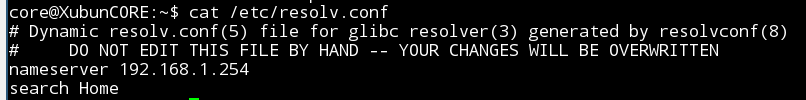
\includegraphics[width=0.7\textwidth]{images/resolv.png}  
    \caption{/etc/resolv.conf}
    \label{fig:resolv}
\end{figure}
O ficheiro /etc/resolv.conf contém as informações relativas aos servidores
de DNS.

\section{Pergunta b}
\textbf{Os servidores www.sapo.pt. e www.yahoo.com. têm endereços IPv6? Se sim,
quais?}\\
Para sabermos quais são os endereços IPv6 dos servidores, utilizamos o comando
host.

\begin{figure}[H]
    \centering 
    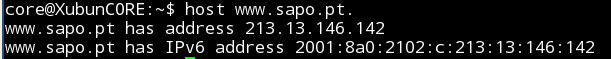
\includegraphics[width=0.7\textwidth]{images/sapopt.png}  
    \caption{sapo.pt}
    \label{fig:sapopt}
\end{figure}
Como podemos reparar na figura \ref{fig:sapopt}, o servidor www.sapo.pt tem o endereço 
IPv6 2001:8a0:2102:c:213:13:146:142,

\begin{figure}[H]
    \centering 
    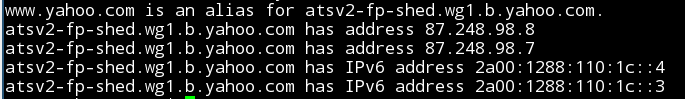
\includegraphics[width=0.7\textwidth]{images/yahoocom.png}  
    \caption{yahoo.com}
    \label{fig:yahoocom}
\end{figure}
O servidor www.yahoo.com tem o endereço IPv6 2a00:1288:110:1c, como é
possível verificar na figura \ref{fig:yahoocom}.

\section{Pergunta c}
\textbf{Quais os servidores de nomes definidos para os domínios: “uminho.pt.”,
“pt.” e “.”?}
\begin{figure}[H]
    \centering 
    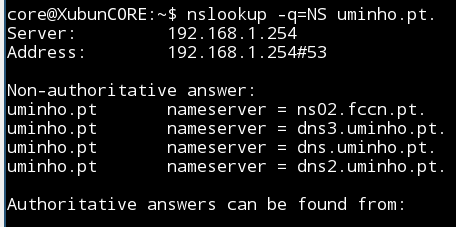
\includegraphics[width=0.5\textwidth]{images/uminhopt.png}  
    \caption{uminho.pt}
    \label{fig:uminhopt}
\end{figure}
Como podemos observar na figura \ref{fig:uminhopt}, para os servidores de nome 
definidos como "uminho.pt" são dns.uminho.pt.

\begin{figure}[H]
    \centering 
    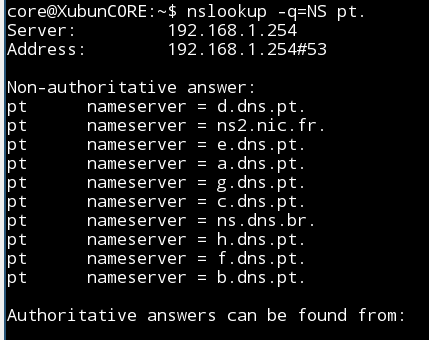
\includegraphics[width=0.5\textwidth]{images/ptponto.png}  
    \caption{pt.}
    \label{fig:ptponto}
\end{figure}
Para os servidores de nome definidos como "pt." são curiosity.dns.pt
(figura \ref{fig:ptponto}).

\begin{figure}[H]
    \centering 
    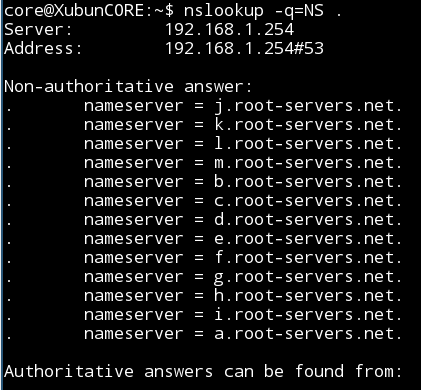
\includegraphics[width=0.5\textwidth]{images/ponto.png}  
    \caption{.}
    \label{fig:ponto}
\end{figure}
E para os servidores de nome definidos como "." são a.root-servers.net
(figura \ref{fig:ponto}).

\section{Pergunta d}
\textbf{Existe o domínio nice.software.? Será que nice.software. é um host ou um
domínio ?}

\begin{figure}[H]
    \centering 
    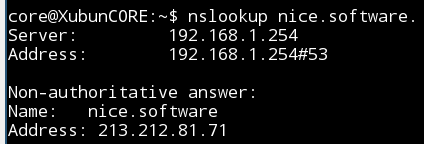
\includegraphics[width=0.8\textwidth]{images/nicesoftware.png}  
    \caption{nice.software.}
    \label{fig:nicesoftware}
\end{figure}
Sendo que, como podemos observar na figura \ref{fig:nicesoftware}, através do nslookup
obtemos endereços de IP, então este dominio existe e é um host.

\section{Pergunta e}
\textbf{Qual é o servidor DNS primário definido para o domínio msf.org.? Este
servidor primário (master) aceita queries recursivas? Porquê?}

\begin{figure}[H]
    \centering 
    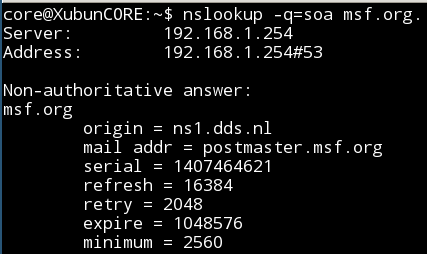
\includegraphics[width=0.8\textwidth]{images/dnsprimario.png}  
    \caption{DNS primário}
    \label{fig:dnsprimario}
\end{figure}
Para obtermos o DNS primário utilizamos o comando nslookup com uma query
do tipo soa. O resultado está apresentado na figura \ref{fig:dnsprimario} e
como podemos ver está definido como ns1.dds.nl.

\begin{figure}[H]
    \centering 
    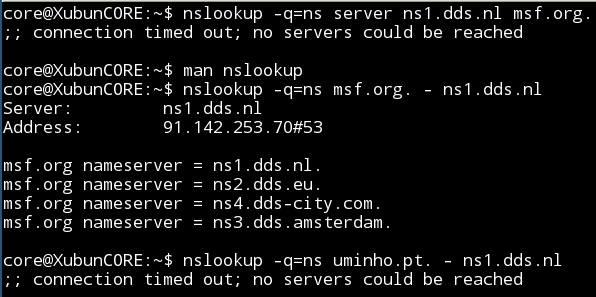
\includegraphics[width=0.8\textwidth]{images/recursivo.png}  
    \caption{teste de recursividade}
    \label{fig:recursivo}
\end{figure}
Com o intuito de testar a recursividade, voltamos a usar o comando nslookup
mas desta vez com o DNS primário. Na figura \ref{fig:recursivo}, não obtivemos
resposta nem do DNS primário para msf.org nem do uminho.pt para o DNS primário.
No entanto, do msf.org para o DNS primário foi obtida uma resposta. Sendo assim
podemos concluir que este não é recursivo.

\section{Pergunta f}
\textbf{Obtenha uma resposta “autoritativa” para a questão anterior.}\\
Não foi possível obter uma resposta autoritativa.

\begin{figure}[H]
    \centering 
    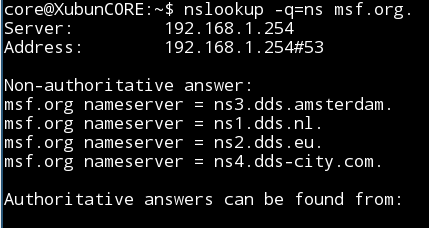
\includegraphics[width=0.8\textwidth]{images/autoritativa.png}  
    \caption{Tentativa de resposta autoritativa}
    \label{fig:autoritativa}
\end{figure}

\section{Pergunta g}
\textbf{Onde são entregues as mensagens de correio eletrónico dirigidas aos
presidentes marcelo@presidencia.pt e bolsonaro@casacivil.gov.br?}\\
Como é possível ver na figura \ref{fig:presidencia.pt}, as mensagens são
entregues nos servidores mail1.presidencia.pt e mail2.presidencial.pt, 
sendo entregues preferencialmente no primeiro por o grau de preferência
ser superior.

\begin{figure}[H]
    \centering 
    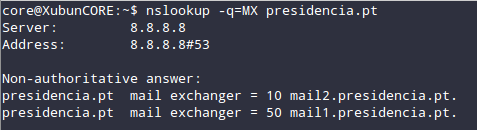
\includegraphics[width=0.8\textwidth]{images/presidencia_pt.png}  
    \caption{presidencia.pt}
    \label{fig:presidencia.pt}
\end{figure}
Relativamente ao Bolsonaro, observando a figura \ref{fig:casacivil.gov.br},
as mensagens são entregues nos servidores esa01.presidencia.gov.br e 
esa02.presidencia.gov.br, sendo também entregues preferencialmente no primeiro
devido ao grau de preferência.

\begin{figure}[H]
    \centering 
    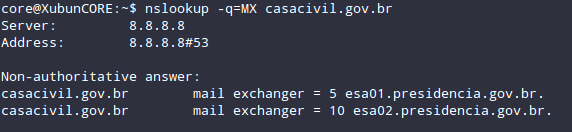
\includegraphics[width=0.8\textwidth]{images/casacivil_gov_br.png}  
    \caption{casacivil.gov.br}
    \label{fig:casacivil.gov.br}
\end{figure}

\section{Pergunta h}
\textbf{Que informação é possível obter, via DNS, acerca de whitehouse.gov?}\\
Para obter o maior número de informações, via DNS, acerca de whitehouse.gov
utilizamos o comando nslookup e o resultado está presente na figura 
\ref{fig:www.whitehouse.gov}.

\begin{figure}[H]
    \centering 
    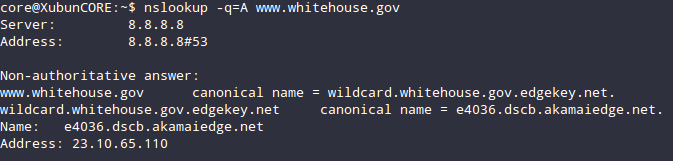
\includegraphics[width=0.8\textwidth]{images/withehouse_gov.png}  
    \caption{www.whitehouse.gov}
    \label{fig:www.whitehouse.gov}
\end{figure}

\section{Pergunta i}
\textbf{Consegue interrogar o DNS sobre o endereço IPv6
2001:690:a00:1036:1113::247 usando algum dos clientes DNS? Que informação
consegue obter? Supondo que teve problemas com esse endereço, consegue obter um
contacto do responsável por esse IPv6?}\\
Analisando a figura abaixo, verificamos que é possível interrogar o DNS usando o
cliente DNS nslookup, no entanto obtemos poucas informações e uma reposta não
autoritativa.

\begin{figure}[H]
    \centering 
    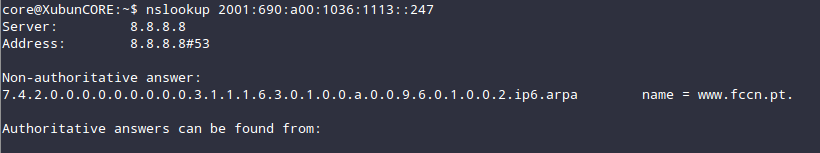
\includegraphics[width=0.8\textwidth]{images/nslookup_ipv6.png}  
    \caption{interrogação nslookup com endereço IPv6}
    \label{fig:nslookup_ipv6}
\end{figure}
Com o objetivo de obter um contacto responsável pelo IPv6, utilizamos
o comando nslookup com uma query do tipo SOA. Observando o resultado
na figura abaixo, reparamos que o contacto responsável por esse IPv6 
é o ns01.fccn.pt.

\begin{figure}[H]
    \centering 
    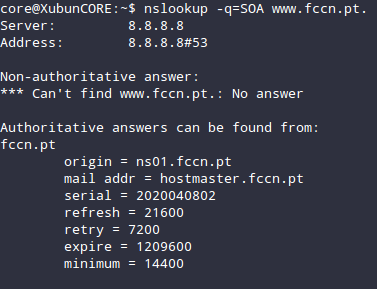
\includegraphics[width=0.7\textwidth]{images/fccn_pt.png}  
    \caption{}
    \label{fig:fccn_pt}
\end{figure}

\section{Pergunta j}
\textbf{Os secundários usam um mecanismo designado por “Transferência de zona”
para se atualizarem automaticamente a partir do primário, usando os parâmetros
definidos no Record do tipo SOA do domínio. Descreve sucintamente esse mecanismo
com base num exemplo concreto (ex: di.uminho.pt ou o domínio cc.pt que vai ser
criado na topologia virtual).}\\
Através do mecanismo de transferência de zona permite que se replique a base de 
dados do servidor primário para o secundário. Para isso, o servidor primário
será requisitado pelo secundário para fazer essa transferência. Analisando os 
campos que nos é mostrado no Record do SOA do dominio di.uminho.pt, conseguirá
aceder ao número de série e parâmetros temporais da base de dados para a sua 
atualização. Se o número de série for o mesmo então teremos que recorrer 
à utilização da query AXFR, conseguindo a informação dos masters. Algo importante
de ser referido é o parâmetro "retry" quando realizamos a query do tipo SOA. 
Esse campo diz nos o tempo em segundos que demorará o slave a voltar a tentar 
caso algo falhe.

\chapter{Parte 2}
\begin{figure}[H]
    \centering 
    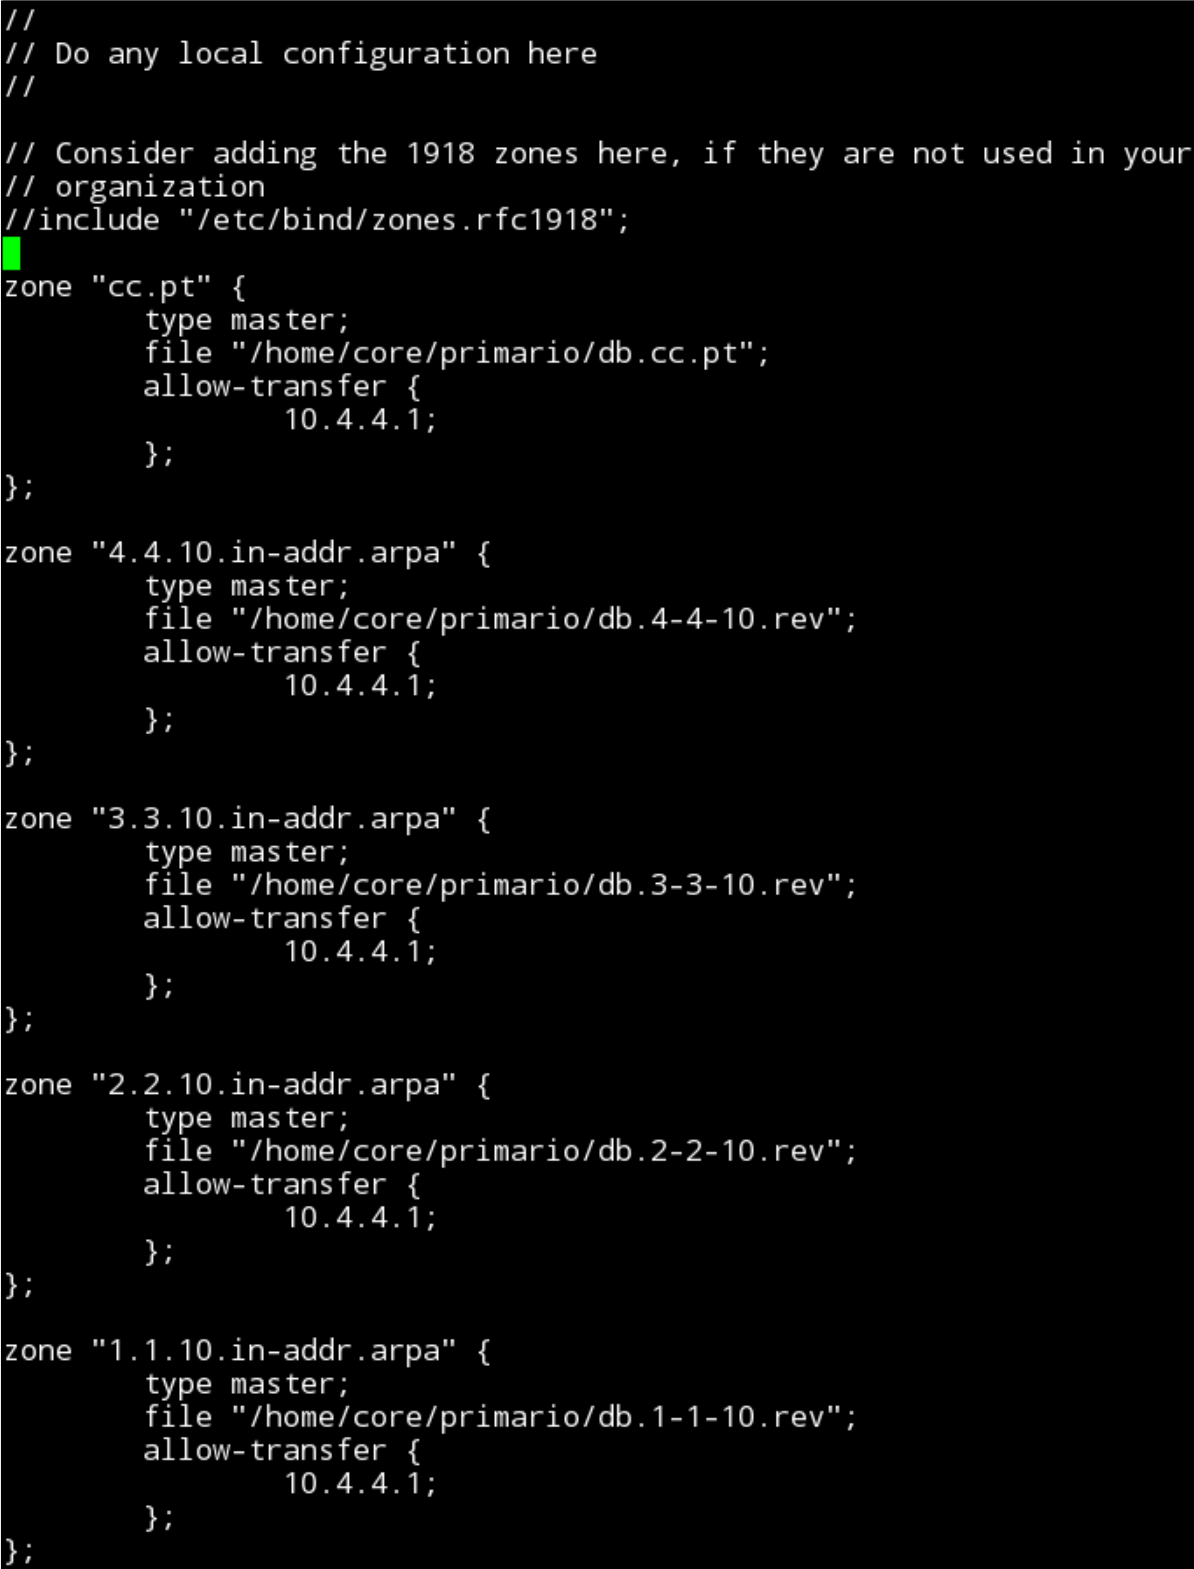
\includegraphics[width=0.8\textwidth]{images/primary_ncl.png}  
    \caption{primario/named.conf.local}
    \label{fig:primary_ncl}
\end{figure}

\begin{figure}[H]
    \centering 
    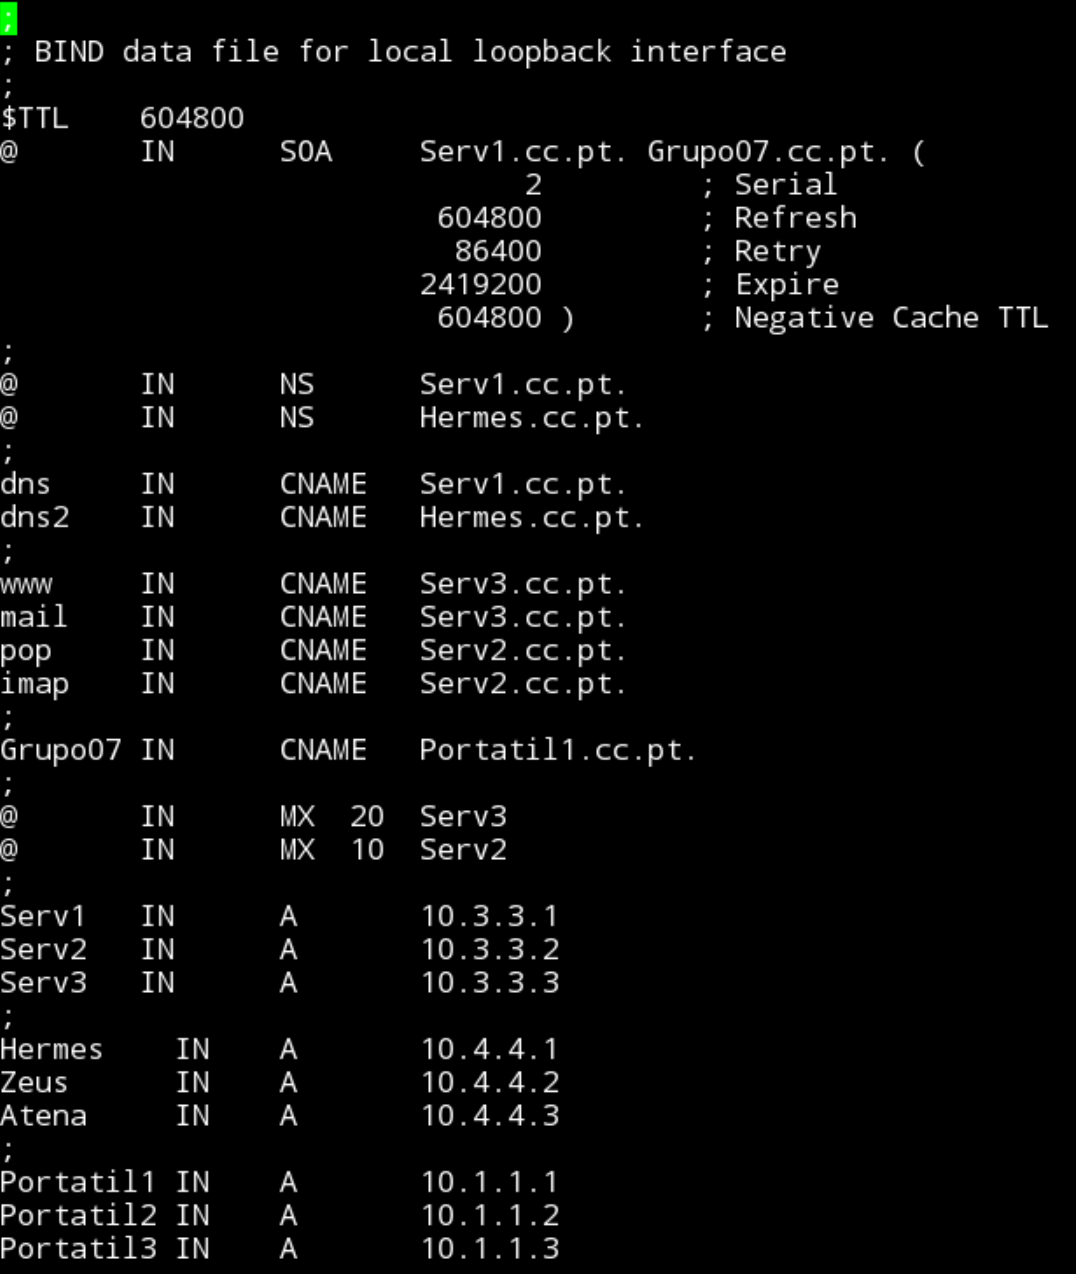
\includegraphics[width=0.8\textwidth]{images/dbccpt.png}  
    \caption{primario/db.cc.pt}
    \label{fig:dbccpt}
\end{figure}

\begin{figure}[H]
    \centering 
    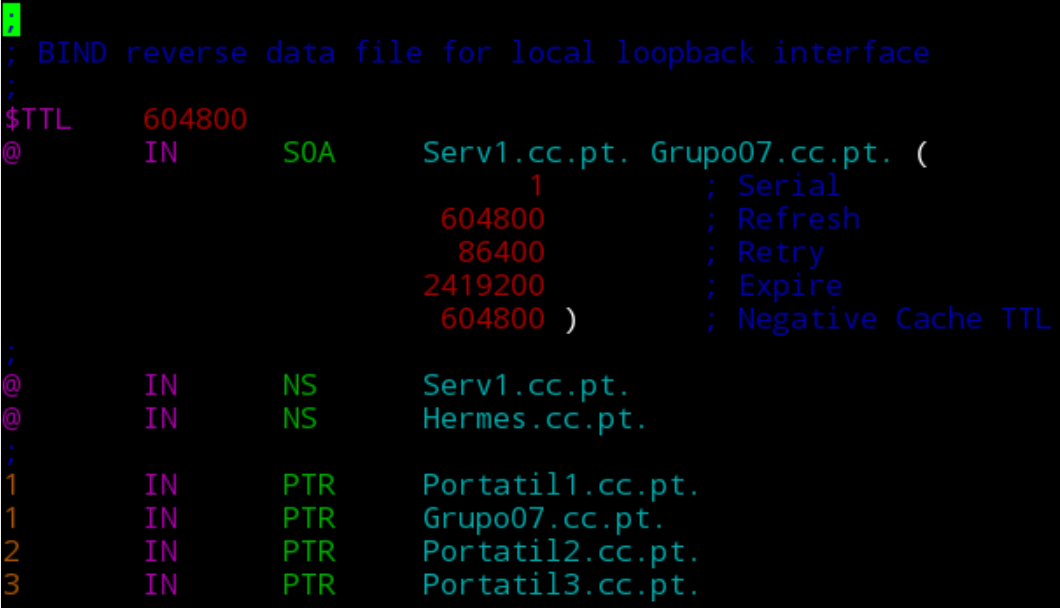
\includegraphics[width=0.8\textwidth]{images/dbrev.png}  
    \caption{primario/db.3-3-10.rev}
    \label{fig:dbrev}
\end{figure}

\begin{figure}[H]
    \centering 
    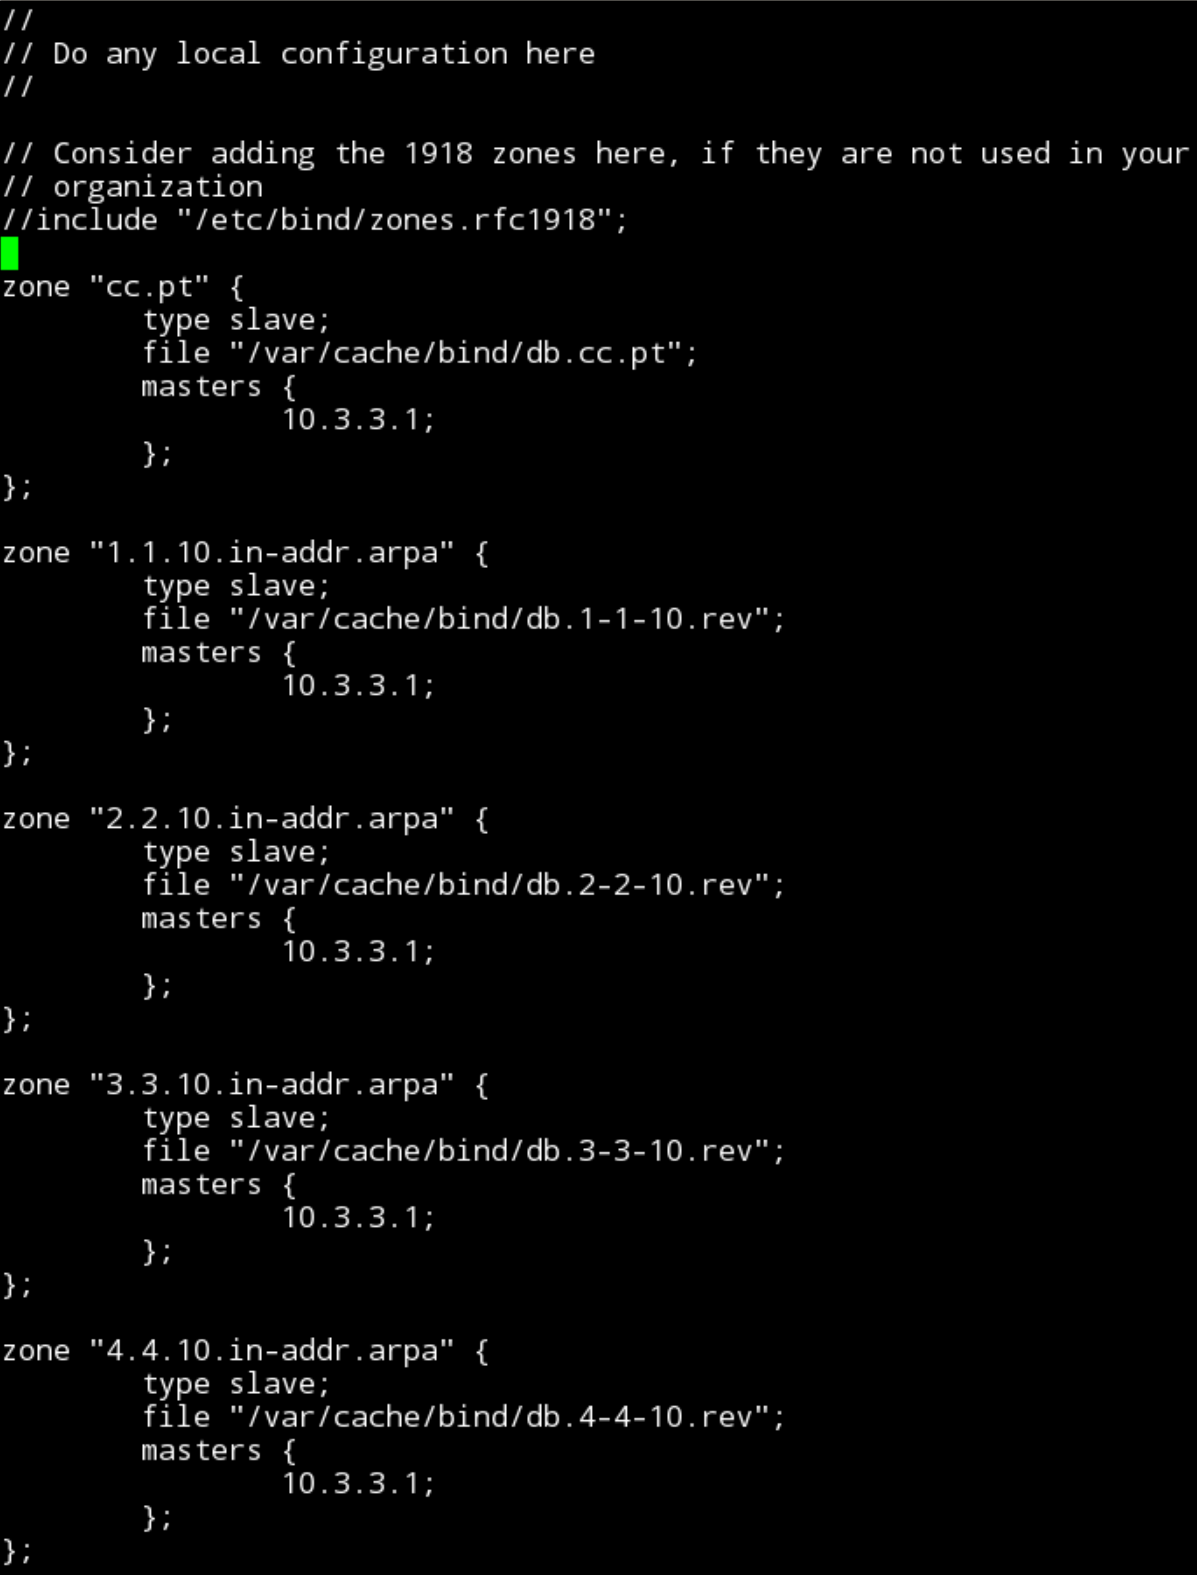
\includegraphics[width=0.8\textwidth]{images/secondary_ncl.png}  
    \caption{secundario/named.conf.local}
    \label{fig:secondary_nncl}
\end{figure}

\section{Testes}

\begin{figure}[H]
    \centering 
    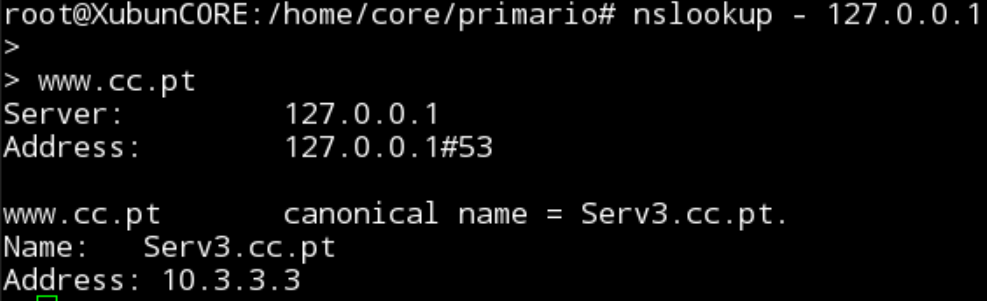
\includegraphics[width=0.8\textwidth]{images/ns_outcore.png}  
    \caption{nslookup fora da topologia core}
    \label{fig:ns_outcore}
\end{figure}

\begin{figure}[H]
    \centering 
    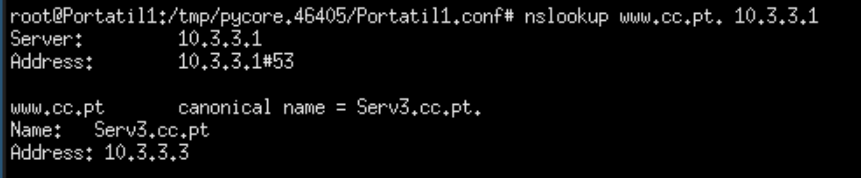
\includegraphics[width=0.8\textwidth]{images/nslookup_portatil1.png}  
    \caption{nslookup feito a partir do portátil 1}
    \label{fig:nslookup_portatil1}
\end{figure}

\begin{figure}[H]
    \centering 
    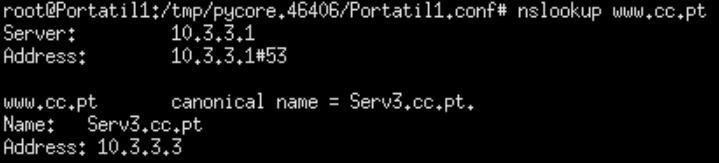
\includegraphics[width=0.8\textwidth]{images/nslookup_resolv.png}  
    \caption{nslookup após alteração do resolv.conf}
    \label{fig:nslookup_resolv}
\end{figure}

\begin{figure}[H]
    \centering 
    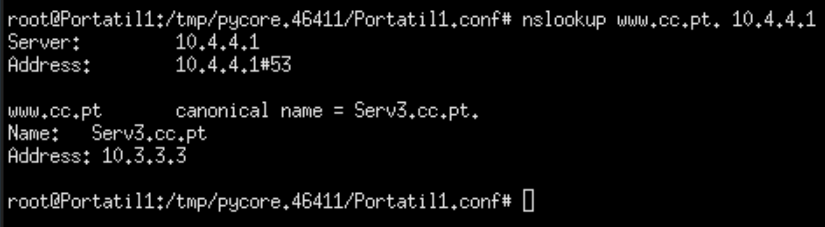
\includegraphics[width=0.8\textwidth]{images/nslookup_secondario.png}  
    \caption{nslookup secundário}
    \label{fig:nslookup_resolv}
\end{figure}

\chapter{Conclusão}

Através da realização deste trabalho foi nos possível reforçar e aprofundar
o nosso conhecimento relativamente à área de serviço de resolução de nomes 
(DNS). No decorrer desta TP foi nos pedido para colocar em prática os 
conceitos aprendidos nas aulas teóricas.
Comparando as duas partes deste trabalho prático, a que se mostrou mais 
difícil de realizar foi a segunda parte, pois foi o primeiro contacto que
tivemos com esta área. Contudo, achamos que conseguimos realizar todas as
tarefas com sucesso sendo que todas as funcionalidades estão implementadas.

\end{document}
